% $Id: calculations-two-prongs.tex 516 2019-04-15 15:01:34Z gsoyez $
\chapter{Two-prong tagging with jet shapes}\label{chap:calc-two-prongs}

 Two-prong taggers aim at
discriminating massive objects that decay into two hard QCD partons
(usually quarks), from the background of QCD jets. This signal is
often an electroweak boson (H/W/Z) but it can also be a new
particle (see Chapter~\ref{searches-measurements} for examples).

Our goal in this chapter is two-folded and it closely follows what was
done in the previous chapter for quark-gluon tagging. First, we want to
give a brief insight into analytic properties of two-prong taggers,
mainly selecting a few representative substructure tools and comparing their
behaviour in Monte Carlo simulations with analytic results. Then, we
will perform a comparative Monte Carlo study of the taggers
discriminating properties, assessing both their performance and their
resilience against non-perturbative effects. 

%%========================================================================
\section{A dive into analytic properties}\label{sec:two-prongs-analytic}

Two-prong taggers used for Run-II of the LHC tend to combine two major
ingredients: a two-prong finder also acting as a groomer, and a cut on
a jet shape for radiation constraint. 
%
Since groomers have already been extensively discussed in
Chapter~\ref{calculations-substructure-mass}, in this chapter we are going to focus on
the understanding of jet shapes and of their
interplay with grooming.
%
Note that a variety of jet shapes can be used in the context of tagging
two-pronged boosted objects: Y-splitter, $N$-subjettiness, ECFs,
pull, and so on.  We will only select a few for our discussion.
 
While computations for groomers and prong-finders, such as the
modified MassDrop Tagger or \SD, have seen a lot of
development towards precision calculations in the last few years and
one can say that they are under good analytic control, the
situation for jet shapes is more complex.
%
This can be understood as follows: imagine one wants to tag a boosted
object around a mass $M_\text{X}$; one would typically first require that the jet
mass (groomed or ungroomed) is in a window close to $M_\text{X}$ and then
that the cut on the jet shape is satisfied; for QCD jets, which constitute the background, this means that we need to consider at least two emissions inside the jet --- one
setting the jet mass, the second setting the value of the shape --- so
calculations for the QCD background will start at order $\alpha_s^2$ in
the perturbative expansion, compared to $\alpha_s$ for groomers or
quark/gluon taggers.
%
That said, calculations now exist for a range of jet shapes~(see
\eg~\cite{Larkoski:2013eya,Larkoski:2014tva,Larkoski:2015kga,Dasgupta:2015lxh,Larkoski:2017iuy,Napoletano:2018ohv}),
noticeably ECFs and $N$-subjettiness, in both the direct QCD approach
used in this book and in SCET.

To keep the discussion simple, we will assume that, on top of working
in the boosted limit $m\ll p_{t,\text{jet}}$, the cut on the jet shape,
$v<v_\text{cut}$, is also small so we can study the effect of the
shape in the leading-logarithmic approximation.
%
Technically, since we expect signal jets to mostly exhibit  small values of $v$
--- \ie there is less radiation in a signal jet than in QCD background
jets --- this approximation seems reasonable. For practical
phenomenological applications however cuts on jet shapes are not much
smaller than one and so finite $v$ corrections are potentially sizeable.
%
The leading-logarithmic approximation we will adopt in what follows,
treating logarithms of $m/p_{t.\text{jet}}$ and $v_\text{cut}$ (and,
optionally of the grooming $\zcut$ parameter) on an equal footing, is
nevertheless sufficient to capture the main properties of two-prong
taggers and differences between them.

For the purpose of this book, we will focus on three different shapes: the
 $N$-subjettiness ratio $\tau_{21}$, with $\beta=2$, which has a fairly
simple structure and has been used at the LHC (albeit with $\beta=1$). We will then move to the dichroic version of the $\tau_{21}$ ratio (see Eq.~\eqref{eq:def-dichroic}) in order to illustrate how separating the
grooming and prong-finding parts of the tagger could be helpful.
Finally, we will discuss the ECFs $C_2^{(\beta=2)}$ and $D_2^{(\beta=2)}$. The latter in particular shows a very good discriminating power and  it is used at the LHC (albeit with $\beta=1$).

A typical LL calculation involves two steps: (i) compute an
expression for the shape valid at LL and (ii) use it to derive an
expression for the mass distribution with a cut on the jet shape, or
the distribution of the shape itself.
%
The calculations for QCD jets will be followed by a calculation for
signal (W/Z/H) jets and a comparison to Monte Carlo simulations done
using the Pythia8 generator.
%
Note that the analytic calculations below focus on computing the jet
mass distribution imposing a cut on the jet shape:
$(\rho/\sigma\,d\sigma/d\rho)_{v<v_\text{cut}}$. We can deduce the
cumulative and differential distribution for the shape itself:
\begin{equation}
  \Sigma(v)=\frac{(d\sigma/d\rho)_{v<v_\text{cut}}}
                 {(d\sigma/d\rho)_{\text{no cut}}}
  \qquad\text{ and }\qquad
  \frac{v}{\sigma}\frac{d\sigma}{dv} = v\frac{d\Sigma}{dv}.
\end{equation}
The background efficiency in a given mass window can also be obtained
from the mass distribution with a cut on the shape via
\begin{equation}
  \epsilon_B(\rho_\text{min},\rho_\text{max};v_\text{cut})
  =\int_{\rho_\text{min}}^{\rho_\text{max}} d\rho \left.\frac{d\sigma}{d\rho}\right|_{v<v_\text{cut}}.
\end{equation}

\subsection{$N$-subjettiness $\tau_{21}^{(\beta=2)}$ ratio}

\paragraph{Approximate $\tau_{21}$ value at LL.}
%
To fully specify the definition of the $\tau_{21}$ ratio we are working with, it is not
sufficient to specify the value of the $\beta$ parameter, one also
needs to specify the choice of axes. For our choice of $\beta=2$, it
is appropriate to work either with minimal axes, \ie the axes that
minimise the value of $\tau_N$, or exclusive generalised-$k_t$ axes
with $p=1/\beta=1/2$. 
Let us consider a set of $n$ emissions. For the purpose of our LL
calculation, we can assume that they are strongly ordered in ``mass'' (or to be more precise in their contribution to the mass)
\ie $\rho_1\gg\rho_2\gg\dots\gg\rho_n$, with $\rho_i=z_i\theta_i^2$,
and strongly ordered in energy and angle (\ie, for example,
$\theta_i\gg\theta_j$ or $\theta_i\ll\theta_j$ for any two emissions
$i$ and $j$).
%
For the sake of definiteness, let us work with axes defined using the
generalised-$k_t$~($p=1/2$) exclusive subjets.
%
We should thus first go through how our set of emissions is clustered.
%
The generalised-$k_t$ clustering will proceed by identifying the
smallest $d_{ij}=\text{min}(z_i,z_j)\theta_{ij}^2$ distance.
%
Using $i=0$ to denote the leading parton and assuming $z_i\ll z_j$, we have
\begin{align}
  d_{i0} & = z_i\theta_i^2 = \rho_i,\\
  d_{ij} & = z_i\theta_{ij}^2
           \approx z_i\,\text{max}(\theta_i^2,\theta_j^2)
           \ge  z_i\theta_i^2 \equiv \rho_i.\label{eq:tau-genkt-ij-distance}
\end{align}
The overall minimal distance will therefore be the smallest of the
$\rho_i$'s, \ie $\rho_n$. This can be realised in two ways: either the
distance between emission $n$ and the leading parton ($d_{n0}=\rho_n$)
of the distance between emission $n$ and any emission $k$ with
$\theta_k\ll\theta_n$ (for which Eq.~\eqref{eq:tau-genkt-ij-distance}
gives $d_{nk}\approx\rho_n$). In the second case, we also have
$z_k\gg z_n$. Due to the energy ordering --- and the fact that for
$\beta=2$ recoil effects can be neglected --- after clustering
particle $n$ with either the leading parton or emission $k$, one gets
a situation with the leading parton and emissions $1,\dots,n-1$. The
above argument can then be repeated, clustering particles
$n-1,n-2,\dots,2,1$ successively.
%
This means that the $\tau_1$ axis will be the jet axis --- equivalent
to the leading parton in this case --- and the two exclusive
generalise-$k_t$ axes used for $\tau_2$ will be aligned with the
leading parton and with the largest $\rho_i$ emission, \ie with
emission 1.\footnote{The argument can be extended to the $N$ exclusive
axes used for $\tau_N$ which would be aligned with the leading parton
and with emissions $1,\dots,N-1$.}

With these axes, it is easy to deduce the value of
$\tau_1$ and $\tau_2$ for our set of emissions:
\begin{align}
\tau_1 & = \sum_{i=1}^n z_i\theta_i^2 = \rho \approx \rho_1,\\
\tau_2 & = \sum_{i=1}^n z_i\text{min}(\theta_i^2,\theta_{i1}^2) \approx \rho_2,\label{eq:tau2-LL-value}
\end{align}
where, in the second line, the contribution from emission $1$ vanishes.

Note that the above derivation is slightly incomplete: on top of the
$n$ emissions from the leading parton, we can also have secondary
emissions from the leading emissions $1,\dots,n$, \ie, in our
angular-ordered limit, emissions ``$j$'' from the leading parton $i$
with $z_j\ll z_i$ and $\theta_{ij}\ll\theta_i$.
%
These will not affect the finding of the two axes needed to compute
$\tau_2$ but secondary emissions from emission $1$ can dominate
$\tau_2$. Specifically, an emission with a momentum fraction $z_2$
relative to $z_1$ emitted at an angle $\theta_{21}$ from emission 1
would give
\begin{equation}\label{eq:tau21-value-secondary}
  \tau_{2,\text{secondary}} \approx z_1 z_2 \theta_{12}^2\qquad\text{\ie}\quad
  \tau_{21,\text{secondary}} \approx z_2\frac{\theta_{12}^2}{\theta_1^2}.
\end{equation}
% 
Another way to view this is to consider that the two axes used to
compute $\tau_2$ define a partition of the jet in two subjets (one
around the leading parton, the second around emission $1$).
%
The total $\tau_2$ is therefore the sum of the individual
contributions from these two subjets, \ie from the sum of
$z_i\theta_{i,\text{axis}}^2$ in these two subjets and the dominant
contribution can come from either subjet.
%
This is in contrast with all the calculations done previously in this
book, which were only sensitive to primary emissions.
%
It should however not come as a surprise since we are discussing tools
which measure the radiation pattern around a two-prong structure so
one should expect a contribution from both prongs.

Note finally that the same result is obtained with the one-pass
generalised-$k_t$ axes or with the minimal axes. However, if we were
to use exclusive $k_t$ axes, which contrary to the above arguments
orders emission's in $z_i\theta_i$, we could have situations where the
emission with the largest $z_i\theta_i$ is different from the emission
with the largest $\rho_i$. This inevitably leads to additional complexity.


\paragraph{LL mass distribution with a cut $\tau_{21}<\tau_\text{cut}$.}
%
Once an expression has been found it is straightforward to understand
the structure of the jet mass distribution with a cut
$\tau_{21}<\tau_\text{cut}$.
%
Since $\tau_{21}$ is given by the second ``most massive'' emission
(either from the leading parton or from the emission which dominates
the jet mass), imposing a cut on $\tau_{21}$ vetoes such emissions,
leaving a Sudakov factor corresponding to virtual emissions in that region of
phase-space.
%
This is represented on the Lund plane in
Fig.~\ref{fig:lund-tau21-plain} and one gets
\begin{align}
  \frac{\rho}{\sigma} \frac{d\sigma}{d\rho}\Big|_{\tau_{21}<\tau_\text{cut}}
  & = \int_0^1 \frac{d\theta_1^2}{\theta_1^2}\frac{dz_1}{z_1}
      \frac{\alpha_s(z_1\theta_1)C_i}{\pi}\rho\delta(\rho-\rho_1)
      \exp[-R_\tau^{\text{(primary)}}-R_\tau^\text{(secondary)}]\label{eq:tau21-plain-mass}\\
  R_\tau^\text{(primary)}
    & =  \int_0^1 \frac{d\theta_2^2}{\theta_2^2}\frac{dz_2}{z_2}
      \frac{\alpha_s(z_2\theta_2)C_i}{\pi}\Theta\Big(\frac{\rho_2}{\rho}>\tau_\text{cut}\Big)\label{eq:tau21-plain-Rprimary},\\
  R_\tau^\text{(secondary)}
    & = \int_0^{\theta_1^2} \frac{d\theta_{12}^2}{\theta_{12}^2}\int_0^1\frac{dz_2}{z_2} \frac{\alpha_s(z_1z_2\theta_{12})C_A}{\pi}\Theta\Big(\frac{z_2\theta_{12}^2}{\theta_1^2}>\tau_\text{cut}\Big),\label{eq:tau21-plain-Rsecondary}
\end{align}
where angles are measured in units of the jet radius $R$ and  the
arguments of the strong couplings are in units of $p_tR$.

\begin{figure}[t]
  \centering
  \subfloat[]{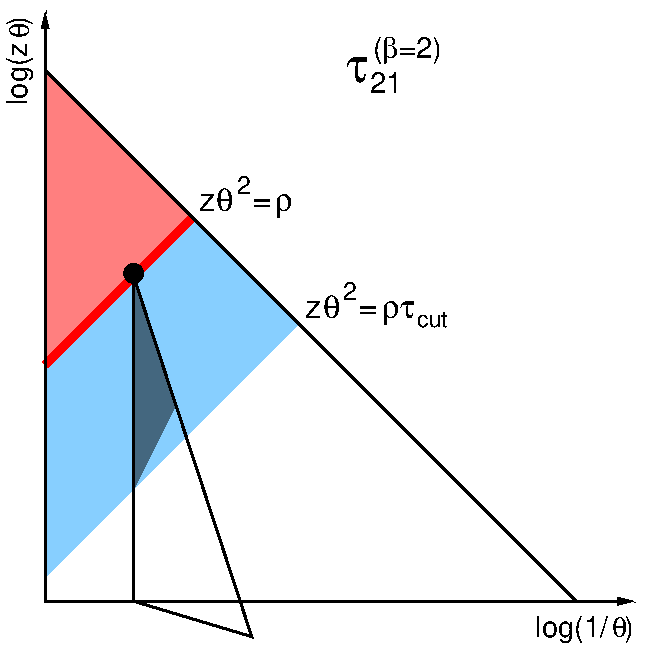
\includegraphics[width=0.48\textwidth]{figures/Lund-tau21.pdf}\label{fig:lund-tau21-plain}}%
  \hfill%
  \subfloat[]{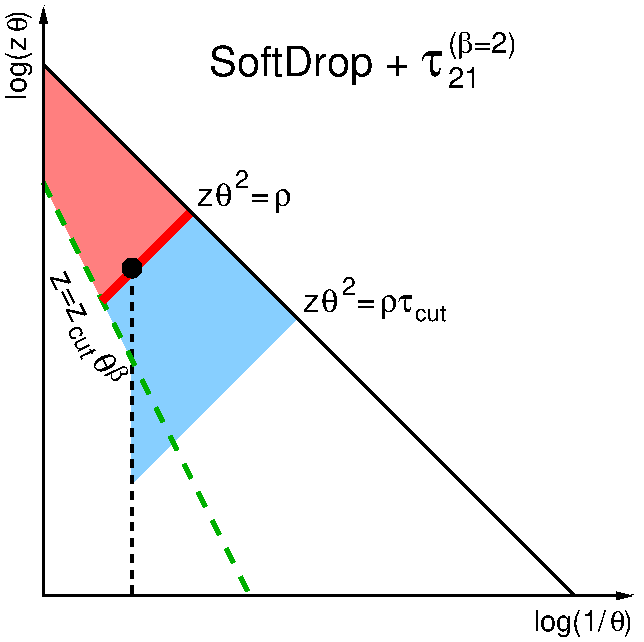
\includegraphics[width=0.48\textwidth]{figures/Lund-tau21-SD.pdf}\label{fig:lund-tau21-SD}}%
  \caption{Lund diagram for the LL mass distribution with a cut on the
    $\tau_{21}$ $N$-subjettiness ratio. The solid red line corresponds
    to the desired jet mass. Real emissions are vetoed in the shaded
    light red region because they would yield a larger mass and in the
    light blue region because they would not pass the cut on
    $\tau_{21}$. The left plot (a) corresponds to the plain jet and the
    right plot (b) to a jet previously groomed with \SD. The left
    plot shows also the plane for secondary (gluon) emissions. An
    identical secondary plane should also be present on the right plot
    but has been omitted for clarity.}\label{fig:lund-tau21}
\end{figure}  

The integration in Eq.~\eqref{eq:tau21-plain-mass} corresponds to the
particle which dominates the jet mass, \ie constrained so that
$\rho=\rho_1$. Eq.~\eqref{eq:tau21-plain-Rprimary} is the Sudakov veto
on primary emissions. It includes a standard jet-mass Sudakov,
$\rho_2>\rho$, from the fact that emission 1 dominates the mass (the
light red region in Fig.~\ref{fig:lund-tau21-plain}), as well as an
additional Sudakov veto $\rho>\rho_2>\rho\tau_\text{cut}$ coming from
the extra constraint on $\tau_{21}$, the light blue region in
Fig.~\ref{fig:lund-tau21-plain}.
%
Finally, Eq.~(\ref{eq:tau21-plain-Rsecondary}) corresponds to the extra
Sudakov veto imposing that secondary emissions with
$\tau_{21}>\tau_\text{cut}$ (cf.~Eq.~(\ref{eq:tau21-value-secondary}))
also have to be vetoed.
%
As before, one can obtain the ``modified'' LL results, including hard
collinear splittings, by setting the upper limits of the $z$ integrations
to $\exp(B_i)$, which is what we do in practical applications below.

In the fixed-coupling approximation, the integrations can be
done analytically, and one obtains
\begin{equation}\label{eq:mass-distrib-tau21-fc}
  \frac{\rho}{\sigma} \frac{d\sigma}{d\rho}\Big|_{\tau_{21}<\tau_\text{cut}}
  \overset{\text{f.c.}}{=}
  \frac{\alpha_s C_i}{\pi} (L_\rho+B_i)
  \exp\Big[-\frac{\alpha_sC_i}{\pi}(L_\rho+L_\tau+B_i)^2
  - \frac{\alpha_sC_A}{\pi}(L_\tau+B_g)^2\Big] ,
\end{equation}
where we have defined
\begin{equation}
  L_\rho = \log(1/\rho)\qquad\text{ and }\qquad
  L_\tau=\log(1/\tau_\text{cut}).
\end{equation}
This has to be compared to the jet mass distribution without the cut
on $\tau_{21}$ which has the same prefactor but only
$\tfrac{\alpha_sC_i}{\pi}(L_\rho+B_i)^2$ in the Sudakov exponent.
%
The cut on $\tau_{21}$ brings an additional Sudakov suppression,
double-logarithmic in $\tau_\text{cut}$ with contributions from both
primary and secondary emissions and, more interestingly, a
contribution proportional to $\log(1/\rho)\log(1/\tau_\text{cut})$,
meaning that with a fixed cut on $\tau_{21}$, the QCD background will
be more suppressed when increasing the jet boost, i.e.\ decreasing $\rho$.
%
We provide more physical discussions below, once we also have
results for the signal and ROC curves.

The calculation of the jet mass with a cut on $\tau_{21}$ can also be
performed for groomed jets, \ie one grooms the jet before measuring
its mass and $\tau_{21}$ on the groomed jet.
%
Here we consider the case of \SD. 
%
As discussed in Sec.~\ref{sec:calc-groomed-mass}, emission 1, which
dominates the \SD mass, has to satisfy the \SD condition and the
associated Sudakov is given by Eq.~(\ref{eq:mMDTSD-radiator-modll}).
%
One small extra complication compared to the case of the \SD jet mass
is that one should
remember that the \SD de-clustering procedure stops once some hard
structure has been found, \ie once the \SD condition is met.
%
Since the de-clustering procedure uses the Cambridge/Aachen jet algorithm, this
means that once the procedure stops, all emissions at smaller angles
are kept, whether or not they pass the \SD condition.

In our LL calculation for $\tau_{21}$, it is sufficient to realise
that one can consider that the \SD procedure keeps all emissions at
angles smaller than $\theta_1$. Thus, the resulting phase-space is depicted in
Fig.~\ref{fig:lund-tau21-SD} and one gets:
\begin{align}
  \frac{\rho}{\sigma} \frac{d\sigma}{d\rho}\Big|_{\tau_{21}<\tau_\text{cut}}^\text{SD}
  & = \int_0^1 \frac{d\theta_1^2}{\theta_1^2}\frac{dz_1}{z_1}
      \frac{\alpha_s(z_1\theta_1)C_i}{\pi}\rho\delta(\rho-\rho_1)
      \,\Theta(z_1>\zcut\theta_1^\beta)
      e^{-R_{\tau,\text{SD}}^\text{(primary)}-R_\tau^\text{(secondary)}}\label{eq:tau21-SD-mass}\\
  R^\text{(primary)}_{\tau,\text{SD}}
    & =  \int_0^1 \frac{d\theta_2^2}{\theta_2^2}\frac{dz_2}{z_2}
      \frac{\alpha_s(z_2\theta_2)C_i}{\pi}\Theta\Big(\frac{\rho_2}{\rho}>\tau_\text{cut}\Big)
      \,\Theta(z_2>\zcut\theta_2^\beta\text{ or }\theta_2<\theta_1).\label{eq:tau21-SD-Rprimary}
\end{align}
The Sudakov corresponding to secondary emissions is the same as for
the plain jet, since all emissions at angles smaller than $\theta_1$
are kept in the groomed jet.
%
Keeping the running-coupling contributions, one finds the following
expressions for the radiators:
\begin{align}
  R^\text{(primary)}_{\tau,\text{SD}}&(\rho,\tau_\text{cut},\theta_1)
  =R_{\text{SD}}^{\text{(LL)}}(\rho\tau_\text{cut}) + \delta
    R_{\tau,\text{SD}}(\rho,\tau_\text{cut},\theta_1)  \\
  \delta R_{\tau,\text{SD}}&(\rho,\tau_\text{cut},\theta_1)
  = \frac{C_i}{2\pi\alpha_s\beta_0^2}\bigg[
    W(1-\lambda_\rho-\lambda_\tau+\lambda_1)
    +\frac{W(1-\lambda_c-(1+\beta)\lambda_1)}{1+\beta}\\
 & -\frac{2+\beta}{1+\beta}W\Big(1-\frac{\lambda_c+(1+\beta)(\lambda_\rho+\lambda_\tau)}{2+\beta}\Big)    
  \bigg]\Theta(\lambda_c+(2+\beta)\lambda_1 > \lambda_\rho+\lambda_\tau)\nonumber\\
  R_\tau^\text{(secondary)}&(\rho,\tau_\text{cut},\theta_1)
  = \frac{C_i}{2\pi\alpha_s\beta_0^2}\bigg[
    W(1-\lambda_\rho-\lambda_{B_g}+\lambda_1)
    +W(1-\lambda_\rho-\lambda_\tau+\lambda_1)\\
  & -2W(1-\lambda_c-\frac{\lambda_\tau+\lambda_{B_g}}{2}+\lambda_1)
    \bigg]\Theta(\lambda_\tau>\lambda_{B_g}),\nonumber
\end{align}
with $\lambda_\rho$ and $\lambda_c$ defined as in
Eq.~(\ref{eq:mMDTSD-radiator-modll}),
$\lambda_\tau=2\alpha_s\beta_0\log(1/\tau_\text{cut})$ and, 
$\lambda_1=2\alpha_s\beta_0\log(1/\theta_1)$ and
$\lambda_{B_g}=-2\alpha_s\beta_0B_g$.
%
$\delta R_{\tau,\text{SD}}$ is the additional contribution from
$\theta_2<\theta_1$ and $z_2<\zcut\theta_2^\eta$.
$R_\tau^\text{(primary)}$ can be easily obtained from
$R^\text{(primary)}_{\tau,\text{SD}}$ by taking the limit
$\beta\to\infty$ and it is nothing else than the plain (ungroomed) jet
mass Sudakov  evaluated at the scale $\rho\tau_\text{cut}$.
Contrary to the fixed-coupling limit, $\delta R_{\tau,\text{SD}}$ and
$R_\tau^\text{(secondary)}$ explicitly depend on $\theta_1$ and the
integration in Eq.~\eqref{eq:tau21-SD-mass} cannot be performed analytically.


\subsection{$N$-subjettiness dichroic $\tau_{21}^{(\beta=2)}$ ratio.}\label{sec:2prongs-analytic-dichroic}

The idea behind dichroic observables arises when combining a prong
finder and a shape constraint.
%
The identification of two hard prongs in a jet, is usually achieved by applying tools
like the mMDT, trimming or pruning to the jet. These algorithms are also active,
(and tight) groomers, meaning that they groom away a large fraction of soft and large-angle radiation in the jet. However, the region of phase-space which is groomed away does carry a lot of information about the radiation pattern, which would be potentially exploited by the shape constraint.
%
The idea is therefore to to compute the shape constraint on a larger,
less tightly groomed jet, that we call the {\em large} jet below. For
shapes which are expressed as a ratio, like $\tau_{21}$, and for
$\beta=2$, the denominator of the shape is a measure of the jet mass
--- recall $\tau_1=\rho$ in the previous section --- which is
naturally computed on the tight jet found by the prong finder,
referred to as the {\em small} jet in what follows.
%
This hints at the following combination
\begin{align}
  \text{mass constraint: }&\text{ use }\rho_{\text{small}},\\
  \text{shape constraint: }&\text{ use }\tau_{21}^{\text{(dichroic)}}=\frac{\tau_{2,\text{large}}}{\tau_{1,\text{small}}}.
\end{align}
We will assume that the small jet is obtained using mMDT with the
condition $z>x_\text{cut}$, and the large jet is either the plain jet
or a \SD jet with positive $\beta$ and a given $\zcut$.
%
We first derive LL analytic results similar to the ones obtained
in the previous section for $\tau_{21}$ and then come back to the
benefits of the dichroic variant.

\paragraph{Approximate $\tau_{21}^\text{(dichroic)}$ value at LL}
%
The value of $\tau_{21}^\text{(dichroic)}$ for a given set of
emissions in a jet can be readily obtained from the results in the
previous section. First, $\tau_{1,\text{small}}$ is
equivalent to the small-jet (dimensionless squared) mass:
$\tau_{1,\text{small}}=\rho_\text{small}$. We will denote by $a$ the
emission that sets the mass of the small jet.

For $\tau_{2,\text{large}}$, we need to use
Eq.~\eqref{eq:tau2-LL-value}, \ie $\tau_{2,\text{large}}$ is dominated
by the emission with the second-largest $\rho_i=z_i\theta_i^2$ in the
large jet. We will therefore denote by $b$ and $c$, the emissions with the
largest and second-largest $\rho_i$ in the large jet,
respectively. With these notations, we get
\begin{equation}
  \tau_{21}^{\text{(dichroic)}} \approx \frac{\rho_c}{\rho_a}\qquad\quad
  \text{($\rho_a$ largest in small, $\rho_c$ $2^\text{nd}$ largest in large)}.
\end{equation}
Note that, contrary to the standard $\tau_{21}$ ratio, the dichroic
ratio can be larger than one.
%
More specifically, three situations can arise: (i) the emission which
dominates the mass of the small jet also dominates the one of the
large jet, \ie $\rho_a=\rho_b>\rho_c$, yielding
$\tau_{21}^{\text{(dichroic)}}<1$; (ii) the emission which dominates
the mass of the small jet is the $2^\text{nd}$ largest in the large
jet, \ie $\rho_b>\rho_a=\rho_c$ yielding
$\tau_{21}^{\text{(dichroic)}}=1$; and (iii) there are at least two
emissions with a larger $\rho_i$ in the large jet than in the small
jet, \ie $\rho_b>\rho_c>\rho_a$ yielding
$\tau_{21}^{\text{(dichroic)}}>1$.
%
It is easy to check that the value of $\tau_{21}^\text{(dichroic)}$ is
always equal or larger than the value of the $\tau_{21}$ ratio obtained 
with approaches frequently used in experimental contexts.
%
 This is a desired feature since increasing the
value of $\tau_{21}$ means rejecting more QCD jets when imposing a
cut.\footnote{As we will see below, this increase of $\tau_{21}$ for
  QCD jets in the dichroic case comes with no modifications for signal
  jets.}


\begin{figure}[t]
  \centering
  \subfloat[]{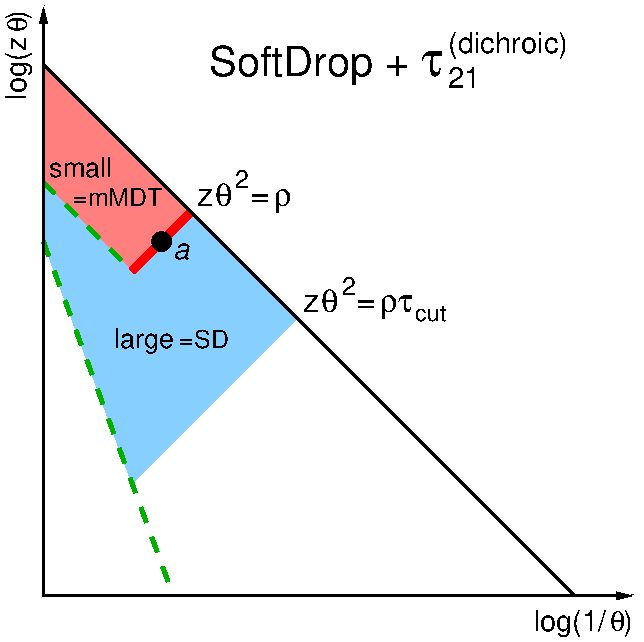
\includegraphics[width=0.48\textwidth]{figures/Lund-tau21-dichroic-SD.pdf}\label{fig:lund-tau21-dichroic-SD}}%
  \hfill%
  \subfloat[]{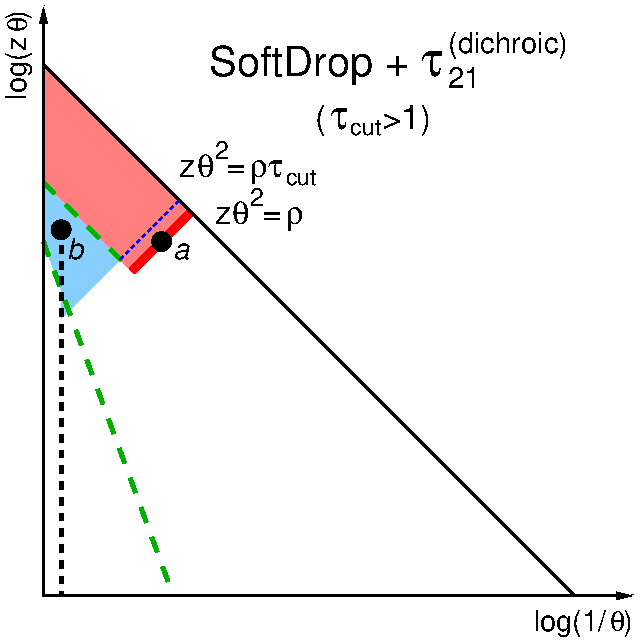
\includegraphics[width=0.48\textwidth]{figures/Lund-tau21-dichroic-SD-gt1.pdf}\label{fig:lund-tau21-dichroic-SD-gt1}}%
  \caption{Lund diagrams for a cut
    $\tau_{21}^{\text{(dichroic)}}<\tau_\text{cut}$, assuming that mMDT
  is used for the small jet and \SD for the large jet. Emissions $a$
  and $b$ are the emissions with the largest $z_i\theta_i^2$ in the
  mMDT and \SD jet respectively. The shaded red region corresponds to
  the vetoed region from the requirement on the (small) jet mass, and
  the shaded blue region is the extra Sudakov veto from the constraint
  on $\tau_{21}^{\text{(dichroic)}}$.
  %
  Figure (a) corresponds to a cut
  $\tau_\text{cut}<1$ for which emissions $a$ and $b$ are identical.
  % 
  Figure (b) corresponds to $\tau_\text{cut}>1$, where one has an
  emission $\rho_b$ in the large jet such that $\rho_b>\rho$ and one
  has to veto real emissions with $z\theta^2>\rho\tau$.
  %
  In both cases, we omitted a contribution from secondary emissions
  for readability. It corresponds to a secondary plane originating
  from emission $a$ (resp. $b$) in case (a) (resp. (b)), with a
  Sudakov veto extending down to $z\theta^2=\rho\tau_\text{cut}$ with
  $z$ measured with respect to the initial
  jet.}\label{fig:lund-dichroic-tau21}
\end{figure}  

\paragraph{LL mass distribution with a cut $\tau_{21}^\text{(dichroic)}<\tau_\text{cut}$.}
%
The calculation of the jet mass distribution with a cut on
$\tau_{21}^\text{(dichroic)}$ has to be separated in the same three
possible of mass orderings as before, corresponding to
$\tau_{21}^\text{(dichroic)}$smaller, equal or larger than $1$.
%
The three situations are represented in
Fig,~\ref{fig:lund-dichroic-tau21} for the case where the large jet
has been groomed with \SD using a positive $\beta$.

The case of a cut $\tau_\text{cut}<1$ is the most interesting as it is
the situation relevant for phenomenology --- the other cases would, as we
show below, also kill the signal --- and where the effect of adopting
a dichroic ratio can be explicitly seen. As for the case of the
standard $\tau_{21}$, one as to integrate over the emission $a$ which
dominates the small jet mass and veto any additional real emission
which would give a value of $\tau_{21}^\text{(dichroic)}$ larger than
$\tau_\text{cut}$, \ie any emission in the large jet with
$z\theta^2>\rho_a\tau_\text{cut}$. This gives
\begin{equation}\label{eq:distrib-tau21dichroic-less1}
  \frac{\rho}{\sigma} \frac{d\sigma}{d\rho}\Big|_{\tau_{21}<\tau_\text{cut}}^\text{dichroic}
  \overset{\tau_\text{cut}<1}{=}
  \int_0^1 \frac{d\theta_a^2}{\theta_a^2}\frac{dz_a}{z_a}
  \frac{\alpha_s(z_a\theta_a)C_i}{\pi}\rho\delta(\rho-\rho_a)
  \,\Theta(z_a>x_\text{cut})
  e^{-R_{\tau,\text{SD}}^\text{(primary)}-R_\tau^\text{(secondary)}},
\end{equation}
with $R_{\tau,\text{SD}}^\text{(primary)}$ and
$R_\tau^\text{(secondary)}$ again given
by~(\ref{eq:tau21-SD-Rprimary}) and~(\ref{eq:tau21-plain-Rsecondary}).
%
Compared to Eq.~(\ref{eq:tau21-SD-mass}), one clearly sees that the
lower bound of the $z_a$ ($z_1$ in~(\ref{eq:tau21-SD-mass}))
integration has been increased, corresponding to a reduction of the
QCD cross-section in the dichroic case.

For completeness, we briefly discuss the case $\tau_\text{cut}\ge 1$.
%
Situations with zero or one emissions in the large jet with
$\rho_b>\rho$ give $\tau_{21}^\text{(dichroic)}\le 1$ and are
therefore accepted. For situations with (at least) two emissions
$\rho_b>\rho_c>\rho_a$, one only accepts the cases with
$\rho_c/\rho<\tau_\text{cut}$.
%
Thus, the only situation which has to be vetoed is
$\rho_b>\rho_c>\rho\tau_\text{cut}$.

This can be reorganised in a slightly more convenient way.
%
First, if there is no emission $\rho_b$ with $\rho_b>\rho\tau_\text{cut}$, the
veto condition cannot be satisfied, meaning the case always
contributes to the cross-section.
%
For cases with at least one emission such that $\rho_b>\rho\tau_\text{cut}$, one
needs an additional veto on emissions $c$ such that
$\rho_b>\rho_c>\rho\tau_\text{cut}$.
%
This situation corresponds to
Fig.~\ref{fig:lund-tau21-dichroic-SD-gt1}.
%
If one assumes that the small jet is obtained using mMDT and the large
jet using \SD, and if we denote by $R_\text{out}$ the radiator
corresponding to the region in the large jet but outside the small one
(\ie the shaded blue region in Fig.~\ref{fig:lund-dichroic-tau21}),
this yields
\begin{align}\label{eq:tau21dichroic-largetau}
  \frac{\rho}{\sigma} \frac{d\sigma}{d\rho}\Big|_{\tau_{21}<\tau_\text{cut}}^\text{dichroic}&
    \overset{\tau_\text{cut}>1}{=}
  \int_0^1 \frac{d\theta_a^2}{\theta_a^2}\frac{dz_a}{z_a}
  \frac{\alpha_s(z_a\theta_a)C_i}{\pi}\rho\delta(\rho-\rho_a)
  \,\Theta(z_a>x_\text{cut})\\
  &\bigg[ e^{-R_\text{out}(\rho\tau_\text{cut})}+\int_0^1 \frac{d\theta_b^2}{\theta_b^2}\frac{dz_b}{z_b}
  \frac{\alpha_s(z_b\theta_b)C_i}{\pi}\Theta(\rho_b>\rho\tau_\text{cut})
  \,\Theta(x_\text{cut}>z_b>\zcut\theta_b^\beta)\nonumber\\
  & \phantom{e^{-R_\text{out}(\rho\tau_\text{cut})}+\int_0^1 \frac{d\theta_b^2}{\theta_b^2}\frac{dz_b}{z_b}\frac{\alpha_s(z_b\theta_b)C_i}{\pi}}
  e^{-R_{\text{out}}(\rho\tau_\text{cut},\rho_b,\theta_b)-R_\tau^\text{(secondary)}(\rho_b,\rho\tau_\text{cut}/\rho_b,\theta_b)}\bigg]\nonumber
\end{align}
In this expression, $R_\text{out}(\rho\tau_\text{cut})$ is trivially
given by
$R_\text{SD}(\rho\tau_\text{cut})-R_\text{mMDT}(\rho\tau_\text{cut})$.
%
In the presence of an emission $b$, one has to be careful that \SD
will keep emissions at angles smaller than $\theta_b$, and therefore
$R_{\text{out}}(\rho\tau_\text{cut},\rho_b,\theta_b)=R_{\tau,\text{SD}}^{\text{(primary)}}(\rho_b,\rho\tau_\text{cut}/\rho_b,\theta_b)-R_\text{mMDT}(\rho\tau_\text{cut})$.
We note that in \eqref{eq:tau21dichroic-largetau}, the integration
over $z_a$ can be done explicitly and gives an overall factor
$R_\text{mMDT}'(\rho)$.
%
Finally, \eqref{eq:tau21dichroic-largetau} does not coincides with
\eqref{eq:distrib-tau21dichroic-less1} when $\tau_\text{cut}\to
1$. This is simply because situations with a single emission
$\rho_b>\rho$ give $\tau_{21}^\text{(dichroic)}=1$, yielding a
discontinuity at $\tau_\text{cut}=1$, or, equivalently, a contribution
to the $\tau_{21}$ distribution proportional to $\delta(\tau_{21}-1)$.

\subsection{Energy-Correlation functions $C_2^{(\beta=2)}$ or $D_2^{(\beta=2)}$}

The last shape we want to discuss is the energy-correlation-function
ratio $D_2$, or, almost equivalently, $C_2$ (which differs from $D_2$
by a factor $\rho$).
%
As before, we first give an analytic expression, valid in the
leading-logarithmic approximation, for the value of $D_2$ for a given
jet. We then compute the mass distribution with a cut
$D_2<D_\text{cut}$.

\paragraph{Approximate $D_2$ value at LL}
%
Consider once again a set of $n$ emissions with momentum fractions
$z_i$ and emitted at angles $\theta_i$ from the parent parton, and
define $\rho_i=z_i\theta_i^2$.
%
We can assume, as before, that the jet mass is dominated by emission
1, \ie the jet mass is $\rho\approx\rho_1$.
%
From Eq.~\eqref{eq:ecf-e3} we then have
\begin{align}
  e_3^{(\beta=2)}
  & = \sum_{i<j<k\in\text{jet}} z_i z_j z_k
      \theta_{ij}^2 \theta_{ik}^2 \theta_{jk}^2
    \approx \sum_{i<j} z_i z_j
      \theta_{ij}^2 \theta_i^2 \theta_j^2\\
  & \approx \sum_{i<j} z_i z_j
      \text{max}(\theta_i^2,\theta_j^2) \theta_i^2 \theta_j^2
    \approx \sum_{i<j} \rho_i \rho_j
      \text{max}(\theta_i^2,\theta_j^2),
\end{align}
where, for the second equality we have used the fact that all
emissions are soft so we can neglect triplets which do not involve the
leading parton, and the third equality comes from the strong angular
ordering between emissions, valid at LL.

For pairs $i,j$ which do not include emission 1, we have, assuming
$\theta_i\ll \theta_j$ , $\rho_i \rho_j \theta_j^2\ll \rho_1 \rho_j
\theta_j^2< \rho_1 \rho_j
\max(\theta_1^2,\theta_j^2)$. These contributions can therefore be
neglected and we have
\begin{equation}
  e_3^{(\beta=2)}
  \approx \rho \sum_{i,\theta_i<\theta_1} \rho_i \theta_1^2 + \rho \sum_{i,\theta_i>\theta_1} \rho_i \theta_i^2.
\end{equation}
At LL accuracy, only one emission, that we will denote by ``2'' will
dominate the sum and we have
\begin{equation}
  e_3 \approx \rho \rho_2 \text{max}(\theta_1^2,\theta_2^2)
  \quad \Rightarrow \quad
  D_2 = \frac{e_3}{e_2^3} \approx \frac{\rho_2}{\rho^2} \text{max}(\theta_1^2,\theta_2^2),
\end{equation}
which has an extra factor $\text{max}(\theta_1^2,\theta_2^2)/\rho$
compared to the $\tau_{21}$ ratio. Alternatively, we can work with
$C_2=\rho D_2$.
%
Note that $D_2$ can be larger than 1 and, in this case, the LL
approximation refers to $C_2\ll 1$ which is dominated by
$\rho_2\ll \rho$ and $\theta_{1,2}^2\ll 1$.

Finally, when imposing a constraint on $D_2$, we are also sensitive to
secondary emissions from 1. A gluon ``2'' emitted with a momentum
fraction $z_2$ (measured with respect to to $z_1$) at an angle $\theta_{12}$ from
1, will give a (dominant) contribution $z_1^2z_2\theta_{12}^2\theta_1^4$
to $e_3$ (taking the leading parton, and emissions 1 and 2 as $i$, $j$
and $k$). We therefore have
\begin{equation}
  D_{2,\text{secondary}} \approx \frac{z_2\theta_{12}^2}{\rho}.
\end{equation}

\paragraph{LL mass distribution with a cut $D_2<D_\text{cut}$}
%
The LL mass distribution with a cut on $D_2$ proceeds as for
$\tau_{21}$ above except that now the constraint on the shape will
impose a Sudakov vetoing emissions for which
$\rho_2 \text{max}(\theta_1^2,\theta_2^2)>\rho^2D_\text{cut}$, with
$\rho_2<\rho$.

The corresponding phase-space is represented in
Fig.~\ref{fig:Lund-D2-all}.
%
We have to consider two regimes. First, for $D_\text{cut}<1$, we have
$\rho^2D/\theta_1^2<\rho$ for any $\rho<\theta_1^2<1$, resulting in
the phase-space represented in Fig.~\ref{fig:Lund-D2}. Then. for
$1<D_\text{cut}<1/\rho$, one can either have $\rho
D_\text{cut}<\theta_1^2$ or $\rho
D_\text{cut}>\theta_1^2$. For the former corresponds one again recovers
Fig.~\ref{fig:Lund-D2}, but for the latter, only the region
$\rho^2D_\text{cut}<\rho_2\theta_2^2<\rho$ (\ie $\theta_2^2>\rho D$),
shown in Fig.~\ref{fig:Lund-D2-large}.

\begin{figure}[t]
  \centering
  \subfloat[]{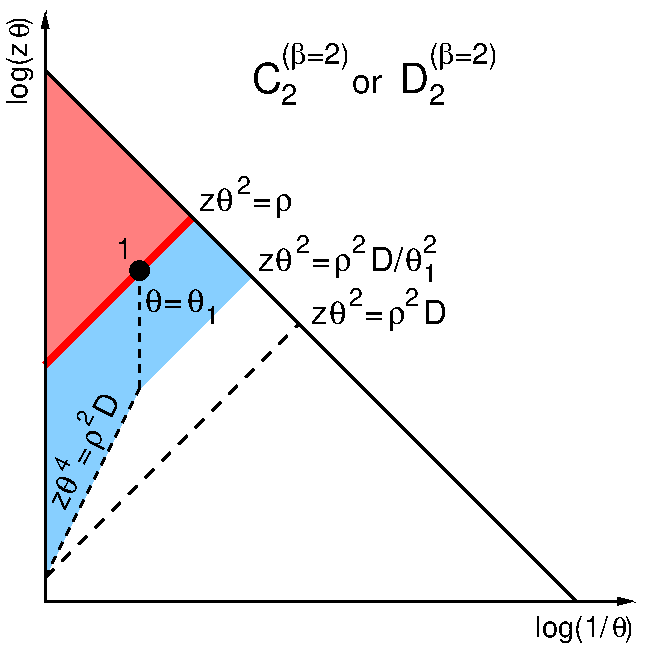
\includegraphics[width=0.48\textwidth]{figures/Lund-D2.pdf}\label{fig:Lund-D2}}%
  \hfill%
  \subfloat[]{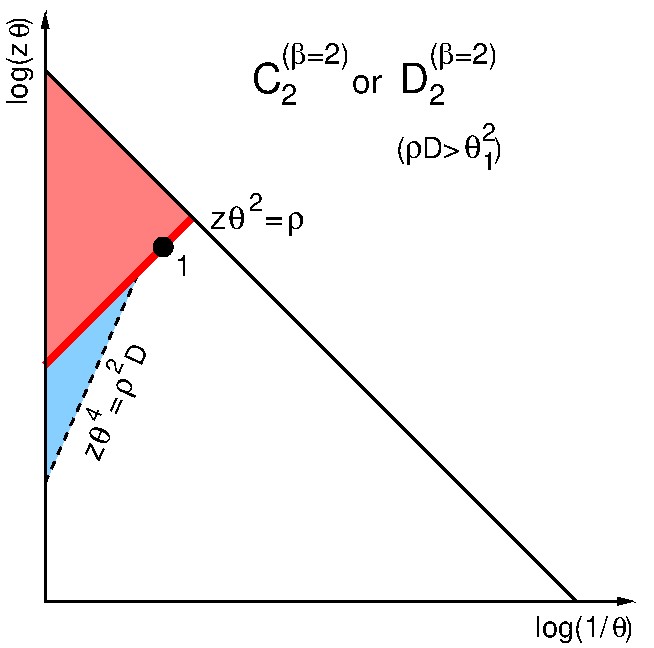
\includegraphics[width=0.48\textwidth]{figures/Lund-D2-large.pdf}\label{fig:Lund-D2-large}}%  
  \caption{Lund diagrams for a constraint $D_2<D_\text{cut}$. For
    $D_\text{cut}<1$, we are always in the situation depicted on
    Fig.~(a), while for $1<D_\text{cut}<1/\rho$, we have either the case
    of Fig.~(a) for $\rho D_\text{cut}<\theta_1^2$ or the case of
    Fig.~(b) for $\rho D_\text{cut}>\theta_1^2$. As above, an extra
    veto for secondary emissions from emission 1 (only in case (a)) is
    not shown for clarity.}\label{fig:Lund-D2-all}
\end{figure}  

The mass distribution with a cut on $D_2$ can be written as 
\begin{align}
  \frac{\rho}{\sigma} \frac{d\sigma}{d\rho}\Big|_{D_2<D_\text{cut}}
  & = \int_0^1 \frac{d\theta_1^2}{\theta_1^2}\frac{dz_1}{z_1}
      \frac{\alpha_s(z_1\theta_1)C_i}{\pi}\rho\delta(\rho-\rho_1)
      \exp[-R_D^\text{(primary)}-R_D^\text{(secondary)}]\label{eq:D2-plain-mass}\\
  R_D^\text{(primary)}
    & =  \int_0^1 \frac{d\theta_2^2}{\theta_2^2}\frac{dz_2}{z_2}
      \frac{\alpha_s(z_2\theta_2)C_i}{\pi}\Theta\Big(\frac{\rho_2}{\rho} \frac{\text{max}(\theta_1^2,\theta_2^2)}{\rho}>D_\text{cut}\Big)\label{eq:D2-plain-Rprimary},\\
  R_D^\text{(secondary)}
    & = \int_0^{\theta_1^2} \frac{d\theta_{12}^2}{\theta_{12}^2}\int_0^1\frac{dz_2}{z_2} \frac{\alpha_s(z_1z_2\theta_{12})C_A}{\pi}\Theta\Big(\frac{z_2\theta_{12}^2}{\rho}>D_\text{cut}\Big).\label{eq:D2-plain-Rsecondary}
\end{align}
For the two cases above, one finds, at LL (including both the
mass and shape vetoes)
\begin{align}
  R_D^\text{(primary)} = \frac{C_i}{2\pi\alpha_s\beta_0^2}
    & \begin{cases}
    \frac{1}{3} W(1-2\lambda_\rho-\lambda_D)
    +\frac{2}{3} W(1-2\lambda_\rho-\lambda_D+\frac{3}{2}\lambda_1)\\
    \qquad -2 W(1-\frac{2\lambda_\rho+\lambda_D-\lambda_1+\lambda_B}{2})
    + W(1-\lambda_B) & \text{if }\rho D<\theta_1^2\\
    \frac{1}{3} W(1-2\lambda_\rho-\lambda_D)
    +\frac{2}{3} W(1-\frac{\lambda_\rho-\lambda_D}{2})\\
    \qquad -2 W(1-\frac{\lambda_\rho+\lambda_B}{2})
    + W(1-\lambda_B) & \text{if }\rho D>\theta_1^2\\    
  \end{cases}\\
  R_D^\text{(secondary)} = \frac{C_A}{2\pi\alpha_s\beta_0^2} &
  \bigg[                                                              
     W\Big(1-2\lambda_\rho-\lambda_D+\frac{3}{2}\lambda_1\Big)
    -2 W\Big(1-\frac{3\lambda_\rho+\lambda_D-2\lambda_1+\lambda_{B_g}}{2}\Big)\nonumber\\
    & + W\Big(1-\lambda_\rho-\frac{\lambda_1}{2}+\lambda_{B_g}\Big)\bigg]
      \Theta(2\lambda_\rho+\lambda_D-\lambda_1>\lambda_{B_g})
\end{align}
where $\lambda_\rho$ and $\lambda_B$ are defined as before and we have
introduced $\lambda_D=2\alpha_s\beta_0\log(1/D_\text{cut})$ and
$\lambda_1=2\alpha_s\beta_0\log(1/\theta_1^2)$.
%
$R_D^\text{(primary)}$ is manifestly continuous at $\rho D=\theta_1^2$.

As for the case of $\tau_{21}$, similar expressions can be obtained
with \SD. In this case, the integration over emission 1 in
Eq.~(\ref{eq:D2-plain-mass}) has to be restricted to the region where
emission 1 passes the \SD condition. Focusing on the case
$\rho<\zcut$, one has ,for a given $z_1\theta_1^2=\rho$,
$z_1>(\zcut^2\rho^\beta)^{\frac{1}{2+\beta}}$ or
$\theta_1<(\rho/\zcut)^{\frac{1}{2+\beta}}$.
%
The Sudakov for primary emissions also gets modified by \SD as one
only needs to veto emissions for which either
$z_2>\zcut\theta_2^\beta$ or $\theta_2<\theta_1$. The veto on
secondary emissions is unchanged compared to the plain-jet case.
%
After some relatively painful manipulations, one gets
\begin{align}
  R_{D,\text{SD}}^\text{(primary)} = R_D^\text{(primary)}
  - \frac{C_i}{2\pi\alpha_s\beta_0^2}
  \bigg[\frac{1}{3}W(1-2\lambda_\rho-\lambda_D)
  +\frac{W(1-\lambda_c)}{1+\beta}\nonumber\\
  -\frac{1}{3}W\Big(1-2\lambda_\rho-\lambda_D+\frac{3}{2}\lambda_1\Big)
  -\frac{1}{1+\beta}W\Big(1-\lambda_c-\frac{1+\beta}{2}\lambda_1\Big)
  \bigg]  
\end{align}
if $\rho D<\theta_1^2$ and  $\rho^2 D< \zcut \theta_1^{4+\beta}$,
\begin{align}
  R_{D,\text{SD}}^\text{(primary)} = R_D^\text{primary)}
  - \frac{C_i}{2\pi\alpha_s\beta_0^2}
  \bigg[\frac{1}{3}W(1-2\lambda_\rho-\lambda_D)
  +\frac{W(1-\lambda_c)}{1+\beta}\nonumber \\
  -\frac{4+\beta}{3(1+\beta)}W\Big(1-\frac{(1+\beta)(2\lambda_\rho+\lambda_D)+3\lambda_c}{4+\beta}\Big)
  \bigg],
\end{align}
if either $\rho D<\theta_1^2$ and $\rho^2 D> \zcut
\theta_1^{4+\beta}$, or  $\rho D>\theta_1^2$ and $\zcut^2 \rho^\beta
D^{2+\beta}<1$, and
%
% If we want to write the 1st case above as the 2nd - a correction
% corresponding to the extra triangle:
%
%   -\bigg[
%   \frac{1}{3}W\Big(1-2\lambda_\rho-\lambda_D+\frac{3}{2}\lambda_1\Big)+\frac{1}{1+\beta}W\Big(1-\lambda_c-\frac{1+\beta}{2}\lambda_1\Big)\\
%   -\frac{4+\beta}{3(1+\beta)}W\Big(1-\frac{(1+\beta)(2\lambda_\rho+\lambda_D)+3\lambda_c}{4+\beta}\Big)
%   \bigg]\\
%
\begin{align}
  R_{D,\text{SD}}^\text{(primary)} = R_{\text{SD}}^{\text{(LL)}},
\end{align}
if $\rho D>\theta_1^2$ and $\zcut^2 \rho^\beta D^{2+\beta}>1$.

The first result corresponds to the situation where one has a
contribution similar to $\delta R_{\tau}^\text{(SD)}$ in the
$\tau_{21}$ case, coming from the extra small triangle
$z<\zcut\theta^\beta$, $\theta<\theta_1$. The existence of this
extra region requires $\rho^2 D> \zcut \theta_1^{2+\beta}$.
%
The second result with ``normal'' \SD grooming, covering both
kinematic configurations in Fig.~\ref{fig:Lund-D2-all}.
%
The third result corresponds to the case of
Fig.~\ref{fig:Lund-D2-large} where the shaded blue region is fully
outside the region allowed by the \SD condition, in which case, the
shape cut has no effects and one recovers a \SD mass Sudakov.

This finishes our calculations for our sample of shapes in the case of
QCD jets. Before comparing our results with Monte Carlo simulations,
we briefly discuss the case of signal jets so as to be able to discuss
the performance when tagging $2$-prong boosted objects.


\subsection{Calculations for signal jets}\label{sec:two-prongs-analytic-signal}

In order to be able to study the performance of two-prong taggers
analytically, we also need expressions for signal jets. Generally
speaking, signal jets are dominated by the decay of a colourless heavy
object of mass $m_X$ into two hard partons. Here, we will assume the
decay is in a $q\bar q$ pair, which is valid for electroweak bosons
W/Z/H and for a series of BSM candidates.
%
If the decay happens at an angle $\theta_1$ (measured in units of the
jet radius $R$) and the quark carries a fraction $1-z_1$ of the
boson's transverse momentum, we have
\begin{equation}\label{eq:signal-mass-constraint}
  m_X^2=z_1 (1-z_1) \theta_1^2 (p_tR)^2
  \qquad\text{\ie}\quad
  \rho_X = \frac{m_X^2}{p_t^2R^2}=z_1 (1-z_1) \theta_1^2.
\end{equation}
Furthermore, we will use index 0 (resp. 1) to refer to the quark
(resp. antiquark).


\begin{figure}
  \centerline{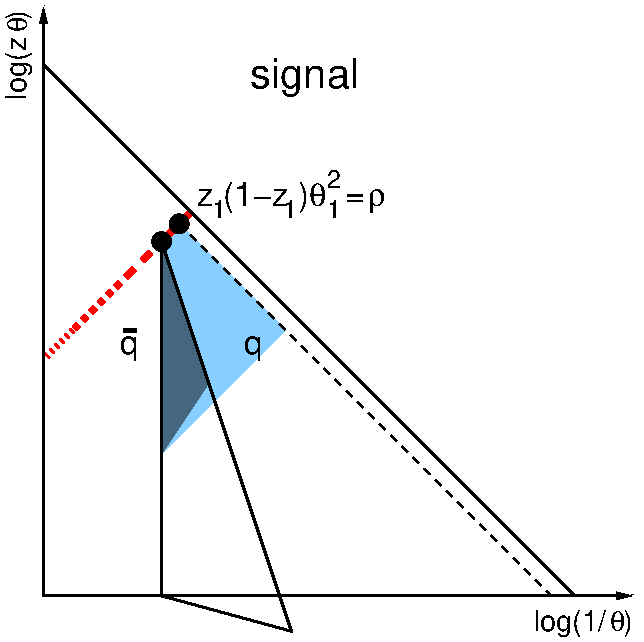
\includegraphics[width=0.48\textwidth]{figures/Lund-tau21_or_D2-signal.pdf}}
  \caption{Lund plane for signal jets. The two solid dots correspond
    to the initial $a\bar{a}$ splitting which satisfies
    $z_1(1-z_1)\theta_1^2=\rho$. A
    % secondary-like
    Lund plane originates from each of the two quarks and the shape
    constraints impose Sudakov vetos (represented as the shaded areas)
    in each of them.}\label{fig:lund-shape-signal}
\end{figure}  

The effect of a cut on a jet shape is similar to what we have just
discussed for QCD jets: it constrains additional radiation in the
jet.
%
The key difference with QCD jets is that now the radiation, is only
coming from the $q\bar q$ dipole. In the collinear limit sufficient
for our purpose here this is equivalent to having two secondary-like
Lund planes associated with the quark and antiquark respectively, as
depicted on Fig.~\ref{fig:lund-shape-signal}.

\paragraph{Calculation of the shape value.}
%
The calculation for a given shape proceeds as before by first
computing an expression for the shape value. Say that emission 2,
emitted at an angle $\theta_{02}$ from the quark (or $\theta_{12}$ from
the antiquark) and carrying a fraction $x_2$ of the jet's transverse
momentum, dominates the shape value (at LL). For the $N$-subjettiness
$\tau_{21}$ ratio, the two axes will align with the quark and
antiquark and we find
%
\begin{equation}
  \tau_2 = x_2 \text{min}(\theta_{02}^2,\theta_{12}^2)
    \quad \Rightarrow\quad
  \tau_{21}\approx\frac{x_2  \text{min}(\theta_{02}^2,\theta_{12}^2)}{\rho}.
\end{equation}
This expression is also valid for the dichroic ratio (just like the
contribution from secondary emission for QCD jets).
%
For ECFs, we get
\begin{equation}
  e_3 = z_1 (1-z_1) x_2 \theta_{01}^2\theta_{02}^2\theta_{12}^2
  \approx \rho\theta_{01}^2 x_2
  \text{min}(\theta_{02}^2,\theta_{12}^2)
  \quad \Rightarrow\quad
  D_2\approx \frac{\theta_{01}^2}{\rho}
  \frac{x_2  \text{min}(\theta_{02}^2,\theta_{12}^2)}{\rho}.
\end{equation}

\paragraph{Signal efficiency.}
%
In the case of signal jets with a fixed jet mass, one should compute
directly the signal efficiency, \ie the fraction of signal jets that
are accepted by the tagger and the cut on the shape.
%
Assuming again that the two hard prongs are identified using \SD as a
prong finder, one can write
%
\begin{equation}
  \epsilon_S(v<v_\text{cut}) = \int_0^1 dz_1 P_X(z_1)
  \Theta(\text{min}(z_1,1-z_1)>\zcut\theta_{01}^\beta)
  %\exp[-R_v^\text{($q$)}(v_\text{cut};z_1)-R_v^\text{($\bar q$)}(v_\text{cut};z_1)]\label{eq:signal-eff-basic}\\
  \,e^{-R_v^\text{($q$)}(v_\text{cut};z_1)-R_v^\text{($\bar q$)}(v_\text{cut};z_1)},\label{eq:signal-eff-basic}\\
\end{equation}
where $P_X(z_1)$ is the probability density for the quark to carry a
fraction $1-z_1$ of the boson's transverse momentum (for simplicity,
we will assume $P_X(z)=1$ in what follows), $\theta_{01}$ is
constrained by Eq.~\eqref{eq:signal-mass-constraint}, and the veto on
radiations in the quark and antiquark prongs takes the form of a
Sudakov suppression, with the two related by a
$z_1\leftrightarrow 1-z_1$ symmetry
$R_v^\text{($\bar q$)}(v;z_1)=R_v^\text{($q$)}(v;1-z_1)$.
%
As already discussed in Sec.~\ref{sec:calc-groomed-mass-signal}, an
important aspect of signal jets is that $P_X$ is finite when $z_1$ or
$1-z_1$ goes to 0.

Note that from the above signal efficiency, one can recover the
differential distribution of the shape value using
\begin{equation}
  \left. \frac{v}{\sigma}\frac{d\sigma}{dv}\right|_\text{signal}
  = \frac{1}{\epsilon_S(\text{no $v$ cut})}
  \left.\frac{d\epsilon_S(v<v_\text{cut})}{d\log(v_{\text{cut}})}\right|_{v_\text{cut}=v}.
\end{equation}

The Sudakov exponents can be computed explicitly for the $\tau_{21}$
ratio and $D_2$.
%
For $\tau_{21}$ (``standard'' or dichroic), we find, using
$x_2=(1-z_1)z_2$
\begin{equation}
  R_v^\text{($\bar q$)}(v;z_1)
  = \int_0^{\theta_{01}^2} \frac{d\theta_{02}^2}{\theta_{02}^2}
  \int_0^1 \frac{dz_2}{z_2}
  \frac{\alpha_s(x_2\theta_{02})C_F}{\pi}
  \Theta((1-z_1)z_2\theta_{02}^2>\rho\tau_\text{cut})
  \Theta((1-z_1)^2z_2\theta_{02}^2<\rho),
\end{equation}
where the last condition of the first line imposes that emission 2
does not dominate the mass.\footnote{This is mostly an artefact of our
  approximations. In the case of signal jets with $z_1\ll 1$, this is
  equivalent to saying that the effect of the shape corresponds to the
  shaded blue region in Fig.~\ref{fig:lund-tau21} which extends up to
  $z\theta^2=\rho$, with the region above corresponding to the
  structure which gives the mass. In practice, this condition is valid
  up to finite squared logarithms of $1-z_1$ when $1-z_1>z_1$, \ie
  well beyond our current accuracy.}
%
At leading logarithmic accuracy, including as well
hard-collinear splittings by imposing $z_2<\exp(B_q)$ as before, one
gets (with $\log(1/\tau)+B_q>0$)
\begin{align}
  R_\tau^\text{($\bar q$)}(v;z_1) \overset{\text{LL}}=
  & \frac{C_F}{2\pi\alpha_s\beta_0^2}\bigg\{
    \bigg[ W\Big(1-\frac{\lambda_\rho-\lambda_z+\lambda_-}{2}-\lambda_B\Big)
        -2 W\Big(1-\frac{\lambda_\rho+\lambda_-+\lambda_\tau+\lambda_B}{2}\Big)
    \nonumber\\
  & + W\Big(1-\frac{\lambda_\rho+\lambda_z+\lambda_-}{2}-\lambda_\tau\Big)\bigg]
    -\bigg[W\Big(1-\frac{\lambda_\rho-\lambda_z+\lambda_-}{2}-\lambda_B\Big)\\
  & -2 W\Big(1-\frac{\lambda_\rho+\lambda_B}{2}\Big)
    + W\Big(1-\frac{\lambda_\rho+\lambda_z-\lambda_-}{2}\Big)\bigg]
    \Theta(\lambda_z-\lambda_->\lambda_B)\bigg\},\nonumber
\end{align}
where $\lambda_z=2\alpha_s\beta_0\log(1/z_1)$ and $\lambda_-=2\alpha_s\beta_0\log(1/(1-z_1))$.

For $D_2$ we find similarly (with $\log(1/\tau)+B_q>\log(z_1^2(1-z_1))$
\begin{align}
  R_D^\text{($\bar q$)}(v;z_1) 
  & = \int_0^{\theta_{01}^2} \frac{d\theta_{02}^2}{\theta_{02}^2}
  \int_0^1 \frac{dz_2}{z_2}
  \frac{\alpha_s(x_2\theta_{02})C_F}{\pi}
  \Theta\Big(\frac{z_2\theta_{02}^2}{z_1}>\rho D\Big)\Theta((1-z_1)^2z_2\theta_{02}^2<\rho)
  \nonumber\\
  & \overset{\text{LL}}= \frac{C_F}{2\pi\alpha_s\beta_0^2}\bigg\{
    \bigg[ W\Big(1-\frac{\lambda_\rho-\lambda_z+\lambda_-}{2}-\lambda_B\Big)
        -2 W\Big(1-\frac{\lambda_\rho+\lambda_z+2\lambda_-+\lambda_D+\lambda_B}{2}\Big)
    \nonumber\\
  & + W\Big(1-\frac{\lambda_\rho+3\lambda_z+3\lambda_-}{2}-\lambda_D\Big)\bigg]
    -\bigg[W\Big(1-\frac{\lambda_\rho-\lambda_z+\lambda_-}{2}-\lambda_B\Big)\\
  & -2 W\Big(1-\frac{\lambda_\rho+\lambda_B}{2}\Big)
    + W\Big(1-\frac{\lambda_\rho+\lambda_z-\lambda_-}{2}\Big)\bigg]
    \Theta(\lambda_z-\lambda_->\lambda_B)\bigg\},\nonumber
\end{align}

These expressions will be compared to Monte Carlo simulations in the
next section where we also discuss key phenomenological observations.

\section{Comparison to Monte Carlo simulations}

In this section, we compare our analytic results to Monte Carlo
simulations obtained with Pythia. For all the Monte Carlo simulations in
this chapter, we have relied on the samples used in the ``two-prong
tagger study'' performed in the context of the Les Houches
Physics at TeV Colliders workshop in 2017 (Section~III.2 of
Ref.~\cite{Bendavid:2018nar}).
%
Background jets are obtained from a dijet sample while signal jets
are obtained from a WW event sample.

In order to streamline our discussion, we focus on a selection of five working
points:
\begin{itemize}
  \setlength\itemsep{0cm}
  \item $\tau_{21}^\text{(SD)}$: \SD jet mass with a cut on
    $\tau_{21}^{(\beta=2)}$ computed on the \SD jet;
  \item $\tau_{21}^\text{(mMDT)}$: mMDT jet mass with a cut on
    $\tau_{21}^{(\beta=2)}$ computed on the mMDT jet;
  \item $\tau_{21}^\text{(dichroic)}$: mMDT jet mass with a cut on
    $\tau_{21}^{(\text{dichroic})}=\tau_2^\text{(SD)}/\tau_1^\text{(mMDT)}$;
  \item $D_2^\text{(SD)}$: \SD jet mass with a cut on
    $D_2^{(\beta=2)}$ computed on the \SD jet;
  \item $D_2^\text{(mMDT)}$: mMDT jet mass with a cut on
    $D_2^{(\beta=2)}$ computed on the mMDT jet.
\end{itemize}
Note that above selection of working points never includes the plain jet. Although using ungroomed jets can show good tagging performances (as expected from the discussion below),
they usually have poor resilience against non-perturbative effects (see next section) and are therefore
less relevant for a comparison to analytic calculations.

\begin{figure}
  \centering
  \subfloat[]{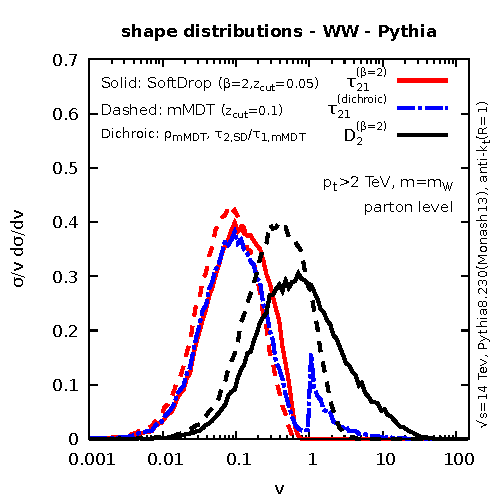
\includegraphics[width=0.48\textwidth]{figures/shapes-distribs-WW-pythia.pdf}\label{fig:shape-distribs-sig-pythia}}%
  \hfill%
  \subfloat[]{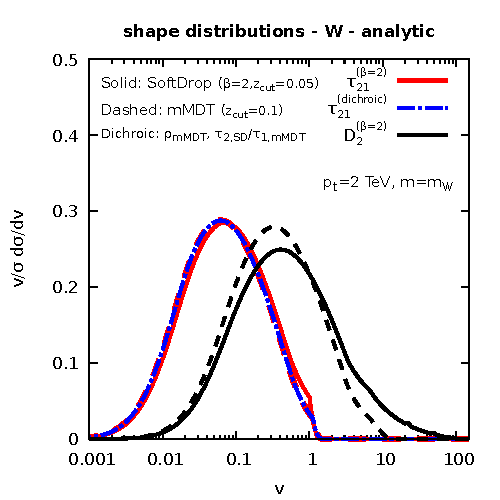
\includegraphics[width=0.48\textwidth]{figures/shapes-distribs-sig-analytic.pdf}\label{fig:shape-distribs-sig-analytic}}\\
  \subfloat[]{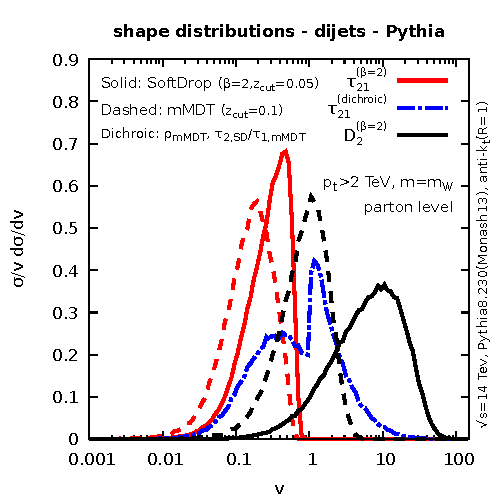
\includegraphics[width=0.48\textwidth]{figures/shapes-distribs-dijets-pythia.pdf}\label{fig:shape-distribs-qcd-pythia}}%
  \hfill%
  \subfloat[]{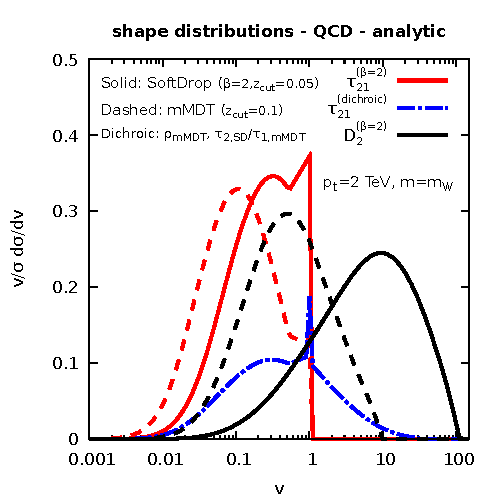
\includegraphics[width=0.48\textwidth]{figures/shapes-distribs-qcd-analytic.pdf}\label{fig:shape-distribs-qcd-analytic}}
  \caption{Distributions for our representative set of shapes as
    obtained from Pythia (left) and from the analytic calculations of
    Sec.~\ref{sec:two-prongs-analytic} (right). The top row
    corresponds to signal (WW) jets while the bottom row shows results for
    background (QCD) jets.}\label{fig:shape-distribs}
\end{figure}


We first focus on the shape distributions, shown for QCD and signal (W) jets in
Fig.~\ref{fig:shape-distribs}.
%
Globally speaking, we see that the main features observed in the Monte
Carlos simulations are well reproduced by our simple analytic
calculations, although the former exhibit distributions that are generally more peaked than the ones obtained with the analytics. 
%
We observe that the signal distribution is, to a large
extend, independent of the level of grooming (\SD or
mMDT). Analytically, this comes from the fact that the grooming
procedure stops at the angle $\theta_{01}$ of the $\text{W}\to q\bar q$
decay, keeping the full radiation inside the two prongs unaffected by
the groomer.
%
The small differences seen in the Pythia simulations are likely due to
radiation outside the $q\bar q$ prongs and to initial-state radiation
which is less efficiently groomed by \SD (with $\beta=2$) than by
mMDT, shifting the former to slightly larger values than the latter.
%
In the case of $D_2$, the differences between the \SD and mMDT results
also involve the fact that the $D_2$ Sudakov has a stronger dependence
on the $p_t$ sharing between the quark and antiquark than $\tau_{21}$.
%
A specific case of this independence of signal distributions to grooming
is that the distribution for the dichroic $\tau_{21}$ ratio is very
close to the ``standard'' ones, again with little differences seen \eg
by the presence of a small peak at $\tau_{21}>1$.

Turning to QCD jets, the situation is clearly different: distributions
shift to smaller values when applying a tighter grooming \ie when
going from \SD to mMDT. This shift is reasonably well reproduced in
the analytic calculation and it is due to the fact that jet shapes are
sensitive to radiations at large angles --- larger than the angle of
the two-prong decay dominating the jet mass --- which is present in
QCD jets, but largely absent in W jets.
%
{\em This has a very important consequence: one expects the tagging
  efficiency to increase for lighter grooming on the jet shape} as the
signal is largely unmodified and the background peak is kept at large
values of the shape.
%
In this context, the case of the dichroic $N$-subjettiness ratio is
also interesting: the dichroic distribution (mixing mMDT and \SD
information) has larger values than both the corresponding \SD and mMDT
distributions.
%
In other words, at small $\tau_{21}$, relevant for tagging purposes,
the dichroic distribution is lower than the \SD and mMDT ones.
%
From an analytic viewpoint, one expects the dichroic distribution to
be smaller than the \SD distribution because, for the same Sudakov
suppression, it imposes a tighter condition on the emission that gives
the mass, and smaller than the mMDT distribution because keeping more
radiation at larger angles increases the Sudakov suppression
(cf.~Figs.~\ref{fig:lund-tau21-SD}
and~\ref{fig:lund-tau21-dichroic-SD}).
%
{\em This is our second important observation: one expects dichroic
  ratios to give a performance improvement.}


One last comment about Fig.~\ref{fig:shape-distribs} is the presence
of peaks for $\tau_{21}^\text{(dichroic)}\gtrsim 1$ in the Pythia
simulation and spikes at $\tau_{21}^\text{(dichroic)}=1$ in our
analytic calculation.
%
As discussed in the analytic calculation of
Sec.~\ref{sec:2prongs-analytic-dichroic}, the cumulative
$\tau_{21}^\text{(dichroic)}$ distribution is discontinuous at
$\tau_{21}^\text{(dichroic)}=1$ and this directly gives a
$\delta(\tau_{21}^\text{(dichroic)}-1)$ contribution to
Fig.~\ref{fig:shape-distribs-qcd-analytic}.\footnote{For readability,
  the  peak has been scaled down on the plot.}
%
Once we go beyond leading logarithmic approximation --- for example,
following the technique introduced in~\cite{Napoletano:2018ohv} ---
this is replaced by a Sudakov peak corresponding to what is seen in the
Pythia simulations from Fig.~\ref{fig:shape-distribs-qcd-pythia}.
%
We also note a kink in the $\tau_{21}$ and
$\tau_{21}^\text{(dichroic)}$ distributions around 0.5. This
corresponds to the point below which secondary emissions start to
contribute, namely $\log(\tau_{21})=B_g$.
%
Since this is in a region where our approximation $\tau_{21}\ll 1$ is
not clearly satisfied, subleading corrections play an important role.


\begin{figure}
  \centering
  \subfloat[]{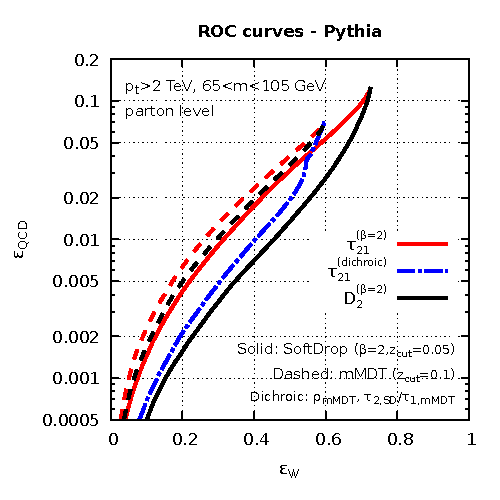
\includegraphics[width=0.48\textwidth]{figures/shapes-rocs-pythia.pdf}\label{fig:shape-rocs-pythia}}%
  \hfill%
  \subfloat[]{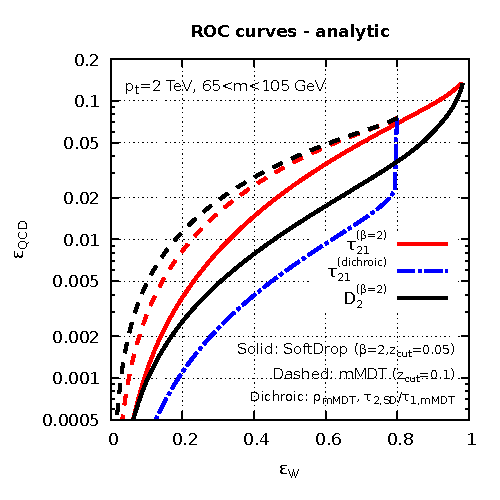
\includegraphics[width=0.48\textwidth]{figures/shapes-rocs-analytic.pdf}\label{fig:shape-rocs-analytic}}%  
  \caption{ROC curves corresponding to our representative set of
    shapes as obtained from Pythia (left) and from the analytic
    calculations (right).}\label{fig:shape-rocs}
\end{figure}

We now turn to a direct analysis of the tagging performance of our
tools with the ROC curves shown on Fig.~\ref{fig:shape-rocs}.
%
Note that the tagging efficiencies include both the effect of the
requirement on the jet mass and of the cut on the jet shape. For signal
jets, we have assumed that the jet mass is exactly the W mass if
the jet passes the $\zcut$ (or \SD) condition on the $\text{W} \to q\bar q$
decay.
%
The two important features highlighted above are indeed seen here:
decreasing the level of grooming results in an increased tagging
performance, as does using dichroic ratios. In the first case, note
that the situation is more delicate at large signal efficiency (close
to the endpoint of the ROC curves corresponding to no constraint on
the jet shape) since one also has to include the effect of the groomer
on constraining the jet mass.
%
Note also that our analytic calculation generally overestimates the
signal efficiency, which is likely due to various oversimplifications
mentioned earlier.

{\em The other important observation (our third) is that a constraint
  on $D_2$ outperforms a constraint on $\tau_{21}$.}\footnote{We refer
  here to the standard definition of $\tau_{21}$. A proper assessment
  of the dichroic ratio would also require using a dichroic version of
  $D_2$ which is done in the next section.}
%
Although there is only a small gain (that the simple analytic
calculation fails to capture) with tight (mMDT) grooming, there is a
clear gain in using $D_2$ when using a looser grooming (\SD) \ie when
opening to larger angles. This is seen in both the analytic
calculation and Monte Carlo simulations.
%
This feature can be explained from our analytic approach.
Based on Fig.~\ref{fig:lund-shape-signal}, fixing the signal
efficiency (say for a given $z_1$ or, equivalently, $\theta_1$) is
equivalent to selecting how much of the radiation is vetoed, \ie fixing
the lower end of the shaded blue region. This, in turns, determines 
the behaviour at small angles ($\theta<\theta_1$) in the case of
background jets. The remaining differences between $\tau_{21}$ and
$D_2$ therefore comes from radiation at angles larger than
$\theta_1$. For the latter, $D_2$ clearly imposes a stronger
constraint (related to its $z\theta^4$ behaviour) than $\tau_{21}$
(with a lighter $z\theta^2$) behaviour,
cf.~Figs~\ref{fig:lund-tau21-plain} and~\ref{fig:Lund-D2}.

To conclude this section, we want to make a final comment on two other
observations emerging from the analytic results.
%
First, in the case of groomers (used here to find the two prongs
dominating the jet mass) we had a strong Sudakov suppression of QCD
jets for a relatively mild (typically $1-2\zcut$) suppression for
signal jets (cf.~Chapter~\ref{calculations-substructure-mass}). In
contrast, imposing a cut on a jet shape yields a Sudakov suppression
for both the background and the signal. This means that if we want to
work at a reasonable signal efficiency, the cut on the shape should
not be taken too small. Our analytic calculations, strictly valid in
the limit $v_\text{cut}\ll 1$ are therefore only valid for
qualitative discussions and a more precise treatment is required for
phenomenological predictions. We refer to
Refs.~\cite{Larkoski:2015kga,Napoletano:2018ohv} for practical
examples.

Our last remark is also {\em our last important point: for a fixed
  mass and cut on the jet shape, the signal efficiency will remain
  mostly independent of the jet $p_t$ but background jets will be
  increasingly suppressed for larger $p_t$.} Analytically, the
associated Sudakov suppression in the signal is independent of
$\rho$. For background jets, the Sudakov exponent increases with the
boost like $\log(1/\rho)$ (cf.~Eq.~\eqref{eq:mass-distrib-tau21-fc},
with a similar result for $D_2$).
%
Note that this dependence on $\rho$ of the background efficiency is
not always desirable. In particular, it might complicate the
experimental estimation of the background, thus negatively impacting searches for
bumps on top of it.
%
An alternative strategy consists of designing a ``decorrelated
tagger''~\cite{Dolen:2016kst} (see description in Sec.~\ref{sec:tools-combinations}), \eg built from $\rho$ and $\tau_{21}$,
yielding a flat background, hence facilitating searches.


%%========================================================================
\section{Performance and robustness}\label{sec:2prongs-perf-robustness}

The last set of studies we want to perform in this chapter is along
the lines of our quality criteria introduced in
Sec.~\ref{sec:performance-intro}, namely looking at two-prong
taggers both in terms of their performance and in terms of their
resilience against non-perturbative effects.
%
An extensive study has been pursued in the context of the Les Houches
Physics at TeV Colliders workshop in 2017 (LH-2017), where a
comparison of a wide range of modern two-prong taggers was
performed. Here, we want to focus on a subset of these results,
highlighting the main features and arguments one should keep in mind
when designing a two-prong tagger and assessing its performance. We
refer to Section~III.2 of Ref.~\cite{Bendavid:2018nar} for additional
details and results.

The study is done at three different values of $p_t$ (500~GeV, 1 and
2~TeV) and here we focus on jets reconstructed with the anti-$k_t$
algorithm with $R=1$ (the LH-2017 study also includes $R=0.8$).
%
Crucially, we are going to discuss in detail the resilience with respect to
non-perturbative effects, including both hadronisation and the
Underlying Event. We refer to the extensive study for a separate
analysis of hadronisation and the UE, as well as for a study of
resilience against detector effects and pileup.

To make things concrete, we consider a wide set of two-prong taggers
which can be put under the form
\begin{equation}
  m_\text{min}<m<m_{max}\qquad
  \text{shape }v=\frac{\text{3-particle observable}}{\text{2-particle observable}}<v_\text{cut},
\end{equation}
where the mass, the two-particle observable and the three-particle observable can
potentially be computed with different levels of grooming.
%
We will focus on four levels of grooming
\begin{itemize}
  \setlength\itemsep{0cm}
\item {\em plain ($p$)}: no grooming,
\item {\em loose ($\ell$)}: \SD with $\beta=2$ and $\zcut=0.05$,
\item {\em tight ($t$)}: mMDT with $\zcut=0.1$,
\item {\em trim}: trimming with $k_t$ subjets using
  $R_\text{trim}=0.2$ and $f_\text{trim}=0.05$,
\end{itemize}
and four different shapes: the $\tau_{21}$ $N$-subjettiness ratio and the
$D_2$, $N_2$ and $M_2$ ECF ratios either with $\beta=1$ or $\beta=2$.
%
\begin{table}[t!]
\begin{center}
\begin{tabular}{| c | c | c |c |c|c|c |c|c | }
  \hline                       
  Notation: $m \otimes n/d$ & $m$ (mass) & $n$ (numerator) & $d$ (denominator)\\
  \hline
  $p    \otimes    p/p$    & plain  &  plain & plain \\
  $\ell \otimes    p/p$    & loose  &  plain & plain \\
  $\ell \otimes    p/\ell$ & loose  &  plain & loose \\
  $\ell \otimes \ell/\ell$ & loose  &  loose & loose \\
  $t    \otimes    p/p$    & tight  &  plain & plain \\
  $t    \otimes \ell/\ell$ & tight  &  loose & loose \\
  $t    \otimes    p/t$    & tight  &  plain & tight \\
  $t    \otimes \ell/t$    & tight  &  loose & tight \\
  $t    \otimes    t/t$    & tight  &  tight & tight \\
  $\text{trim}$            & trim   &  trim  & trim \\
  \hline  
\end{tabular}
\end{center}
\caption{List of the different tagging strategies considered with the
  corresponding level of grooming for the mass, and
  numerator and denominator of the shape variable.}\label{table:lh-grooming-levels}
\end{table}
%
A generic tagger can then be put under the form
\begin{equation}
v\Big[m\otimes\frac{n}{d}\Big],
\end{equation}
where $v$ is one of our three shapes, $m$ is the level of grooming used
to compute the jet mass and $n$ and $d$ are the levels of grooming
used respectively for the numerator and denominator of the shape. We
consider the combinations listed in
Table~\ref{table:lh-grooming-levels}.

In order to study the tagging quality, we impose the reconstructed mass to
be between 65 and 105~GeV and we vary the cut on the jet shape.
%
We select a working point so that the signal efficiency (at truth, \ie
hadron+UE level) is 0.4, which fixes the cut on the jet shape. For
that cut, we can compute both the signal and background efficiencies
at parton level and at hadron+UE level, which allows us to compute the
tagging performance and robustness using the significance
$\epsilon_S/\sqrt{\epsilon_B}$ and resilience $\zeta$ introduced in
Sec.~\ref{sec:performance-intro}.
%
\begin{figure}
  \centering
  \subfloat[]{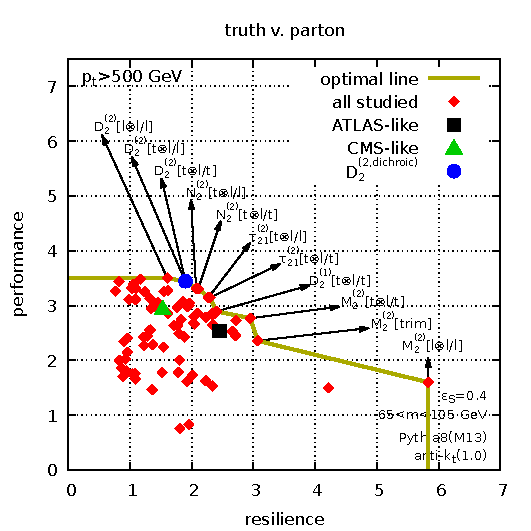
\includegraphics[width=0.48\textwidth,page=1]{figures/lh2017-optimal.pdf}\label{fig:lh2017-optimal-500}}%
  \hfill%
  \subfloat[]{\includegraphics[width=0.48\textwidth,page=3]{figures/lh2017-optimal.pdf}\label{fig:lh2017-optimal-2000}}%  
  \caption{Summary of the performance (significance) v. robustness
    (resilience) of a set of two-prong taggers based on the
    combination of a prong finder and a shape
    cut. }\label{fig:lh2017-optimal}
\end{figure}
%
The resulting tagging qualities are summarised in
Fig.~\ref{fig:lh2017-optimal} for the two extreme $p_t$ values.
%
Each point on the plot represents a different tagger.
%
The ``ATLAS-like'' tagger, i.e. \ trimmed mass with $D_2^{(1)}$ computed on the
trimmed jet), and ``CMS-like'' tagger, i.e.\ mMDT mass with $N_2^{(1)}$ computed on
the mMDT jet, correspond to the working points defined in
Sec.~\ref{sec:tools-combinations}.  The $D_2^\text{(2,dichroic)}$ tagger
corresponds to a working point which appears to show a large
performance without sacrificing too much resilience. This tagger features
$t\otimes \ell/t$ dichroic $D_2$ variable (with angular exponent
$\beta=2$) with the mass computed on the tight jet, the shape
numerator $e_3/(e_e^2)$ computed on the loose jet, and the shape
denominator $e_2$ computed on the tight jet.
%
The plot also shows the line corresponding to the envelope which
maximises resilience for a given performance (and vice versa).


There are already a few interesting observations we can draw from
Fig.~\ref{fig:lh2017-optimal}.
\begin{itemize}
\item As $p_t$ increases, the discriminating power increases as
  well. This can be explained by the fact that when $p_t$ increases,
  the phase-space for radiation becomes larger, providing more
  information that can be exploited by the taggers;
  %
\item The main observations from the previous section still largely
  hold: dichroic variants and variants based on $D_2$ give the best
  performance.
  %
  One possible exception is the case of
  $D_2^{(2)}[\ell\otimes\ell/\ell]$ (\ie both the mass and $D_2$
  computed on the loose (\SD) jet), which shows a slightly larger
  performance than our $D_2^\text{(2,dichroic)}$ working point, albeit
  with a smaller resilience.\footnote{If we were seeking absolute
    performance without any care for resilience, this suggests that
    even looser groomers, possibly combined with a dichroic approach,
    could yield an even greater performance.}
  %
  One aspect which is to keep in mind here is that using a looser
  grooming to measure the jet mass could have the benefit of avoiding
  the $1-2\zcut$ signal efficiency factor before any shape cut is
  applied, of course probably at the expense of more distortion of the
  W peak.
  %
\item Generically speaking, {\em there is a trade-off between
    resilience and performance}.
  %
  This is particularly striking if one looks along the optimal
  line.
  %
  This is an essential feature to keep in mind when designing
  boosted-object taggers: keeping more radiation in the jet (by using
  a looser groomer) or putting tighter constraints on soft radiation
  at larger angles typically leads to more efficient taggers but at
  the same time yields more sensitivity to the regions where
  hadronisation and the Underlying Event have a larger impact, hence
  reducing resilience.
  %
  This is seen both in terms of the shape, when going from $M_2$ to
  $\tau_{21}$ and $N_2$ and then to $D_2$, and in terms of grooming,
  when going from tight to loose jets. 
    %
\item Apart from a few exceptions at relatively lower significance and
  high resilience, the taggers on the optimal are dominated by shapes
  with angular exponent $\beta=2$ rather than the current default at
  the LHC which is $\beta=1$.
  % 
\end{itemize}


\begin{figure}
  \centering
  \subfloat[]{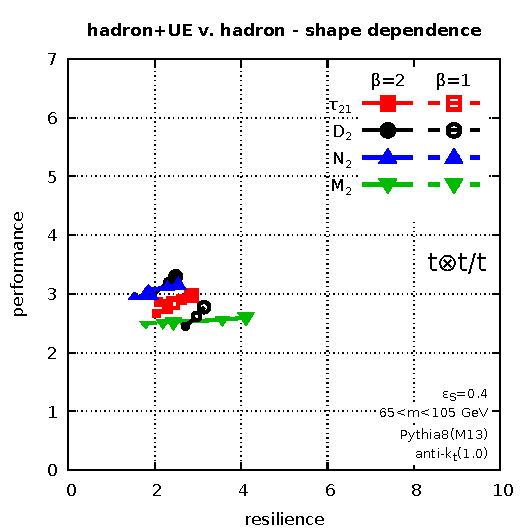
\includegraphics[width=0.48\textwidth,page=1]{figures/lh2017-shape-dependence.pdf}\label{fig:lh2017-shape-ttt}}%
  \hfill%
  \subfloat[]{\includegraphics[width=0.48\textwidth,page=5]{figures/lh2017-shape-dependence.pdf}\label{fig:lh2017-shape-trim}}\\
  \subfloat[]{\includegraphics[width=0.48\textwidth,page=3]{figures/lh2017-shape-dependence.pdf}\label{fig:lh2017-shape-tlt}}%
  \hfill%
  \subfloat[]{\includegraphics[width=0.48\textwidth,page=2]{figures/lh2017-shape-dependence.pdf}\label{fig:lh2017-shape-lll}}%  
  \caption{Dependence of the tagging quality (performance
    versus robustness) on the choice of jet shape.
    %
    Results are shown for different grooming strategies indicated on
    each plot.
    %
    Each curve has three points with increasing symbol size corresponding
    to $p_t=500$~GeV, $1$ and $2$~TeV.
    %
    Each panel corresponds to a different grooming level as indicated on
    the plots.}\label{fig:lh2017-shape}
\end{figure}


\begin{figure}
  \centering
  \subfloat[]{\includegraphics[width=0.48\textwidth,page=2]{figures/lh2017-grooming-dependence.pdf}\label{fig:lh2017-grooming-ttt}}%
  \hfill%
  \subfloat[]{\includegraphics[width=0.48\textwidth,page=6]{figures/lh2017-grooming-dependence.pdf}\label{fig:lh2017-grooming-trim}}\\
  \subfloat[]{\includegraphics[width=0.48\textwidth,page=3]{figures/lh2017-grooming-dependence.pdf}\label{fig:lh2017-grooming-tlt}}%
  \hfill%
  \subfloat[]{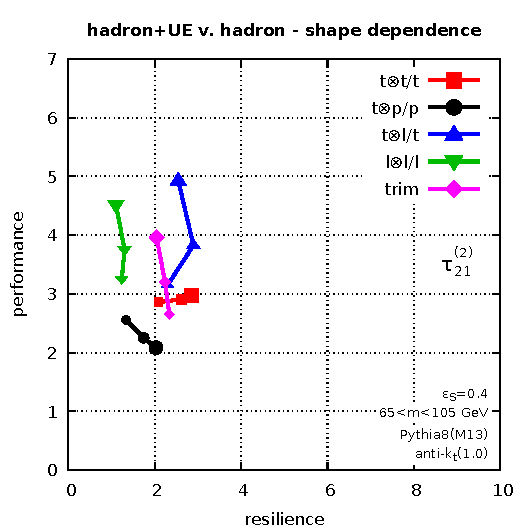
\includegraphics[width=0.48\textwidth,page=1]{figures/lh2017-grooming-dependence.pdf}\label{fig:lh2017-grooming-lll}}%  
  \caption{Dependence of the tagging quality (performance
    versus robustness) on the choice of grooming strategy.
    %
    Results are shown for a representative set of jet shapes.
    %
    Each curve has three points with increasing symbol size corresponding
    to $p_t=500$~GeV, $1$ and $2$~TeV.
    %
    Each panel corresponds to a different choice of shape
    as indicated on the plots.}\label{fig:lh2017-grooming}
\end{figure}

In order to gain a little more insight than what is presented in the
summary plot from Fig.~\ref{fig:lh2017-optimal}, we have extracted a
few representative cases in Fig.~\ref{fig:lh2017-shape}, where each
plot shows different shapes for a fixed grooming strategy and
Fig.~\ref{fig:lh2017-grooming} where each plot shows different
grooming strategies for a fixed shape.
%
All of the key points made above are visible on these plots. We
highlight here a few additional specific examples.

On Fig.~\ref{fig:lh2017-shape}, one sees that the performance of
the taggers increases with $p_t$, with $D_2$ having the best performance,
followed by $\tau_{21}$ and $N_2$ which show a similar pattern, and
$M_2$ which shows a (much) lower performance.
%
With tight grooming, Fig.~\ref{fig:lh2017-shape-ttt}, the phase-space
available for radiation constraint is limited and the differences
between the shapes are not large. Conversely, when opening more
phase-space, \eg Figs.~\ref{fig:lh2017-shape-tlt}
and~\ref{fig:lh2017-shape-lll}, the differences between shapes becomes
more visible.
%
The trade-off between performance and resilience is visible in each
plot, with the exception of $D_2^{(2)}[\ell\otimes\ell/\ell]$ in
Fig.~\ref{fig:lh2017-shape-lll}.
%
We also see that shapes with angular exponent $\beta=2$ show a
better performance than their $\beta=1$ counterparts. In terms of
resilience which can be either smaller (\eg
$D_2^{(2)}[\ell\otimes\ell/\ell]$), similar, or larger (\eg
$N_2^{(2)}[t\otimes\ell]/t$).
%
We note that for plain jets, we would expect $\beta=1$ shapes,
typically behaving like a $k_t$ scale, to be
more resilient than shapes with $\beta=2$, behaving like a mass scale
instead, since they can maximise the available perturbative
phase-space before hitting the hadronisation scale (which corresponds
to a soft $k_t$ scale).
%
And a similar argument hold for the Underlying Event.
%
Conversely, from a perturbative QCD point of view, $\beta=2$ has often
be shown (see \eg \cite{Larkoski:2013eya,Salam:2016yht}) to have a
larger discriminating power.
%
A natural expectation is therefore that once jets are groomed,
non-perturbative these effects are expected to be reduced, giving more
prominence to the perturbative QCD tendency to favour $\beta=2$.
%
Turning finally to Fig.~\ref{fig:lh2017-grooming}, we clearly see for
all four shapes, that using a looser groomer for the shape (either via
the ``all-loose'' $\ell\otimes \ell/\ell$ or the ``dichroic'' $t\otimes\ell/t$
combination) comes with large gains in terms of performance.
%
However, using the plain jet typically shows bad performance, an
effect which can be attributed to an enhanced sensitivity to the
Underlying Event.
%
Comparing the ``all-loose'' and the ``dichroic'' variants, we see that
they show a similar performance, with the dichroic variant having
a larger resilience.


To conclude, we stress once again that, in order to get a complete
picture, the above discussion about performance versus resilience should
be supplemented by a study of the resilience against detector effects
and pileup. Even though we will not do this study here, one can at
least make the educated guess that pileup effects would be reduced by
using a tighter grooming.




%% GS helper for auctex
%%% Local Variables:
%%% mode: latex
%%% TeX-master: "notes"
%%% End:

%  LocalWords:  ECFs SCET Eq eq BSM Houches ECF
